\documentclass[12pt,a4paper]{article}
\usepackage{geometry}
\usepackage[utf8]{inputenc}
\usepackage[spanish]{babel} 
\decimalpoint
\usepackage{a4wide} 
\usepackage{caratula}
\usepackage{afterpage}
\usepackage{hyperref}
\usepackage{xfrac}
\usepackage{xspace}
\usepackage{xargs}
\usepackage{xcolor}
\usepackage{lmodern}
\usepackage[T1]{fontenc}
\usepackage{amsmath,amssymb}
\usepackage{graphicx}
\usepackage{graphbox}
\usepackage{caption}
\usepackage{hhline}
\usepackage{multirow}
\usepackage{listings}
\usepackage{comment}
\usepackage{subcaption} 
\usepackage{ifthen}
\usepackage{fancyhdr}
\usepackage{lastpage}
\usepackage{algorithmicx, algpseudocode, algorithm}


%----------Nuevo comando para hacer un comentario de linea completa en pseudocódigo --------------
\algnewcommand{\LineComment}[1]{\State \(\triangleright\) #1}


%~~~~~~~~~~~~~~~~~~~~~~~~~~~~~~~~~~~~~~~~~~~~~~~~~~~~~~~~~~~~~~~~~~~~~~~~~~~~~~~~~~~~~~~~~~~~~~~~~
%--------Extension del package algorithms para que los algoritmos puedan cruzar la pagina---------

\makeatletter
\newenvironment{breakablealgorithm}
  {% \begin{breakablealgorithm}
   \begin{flushleft}
     \refstepcounter{algorithm}% New algorithm
     \hrule height.8pt depth0pt \kern2pt% \@fs@pre for \@fs@ruled
     \renewcommand{\caption}[2][\relax]{% Make a new \caption
       {\raggedright\textbf{\ALG@name~\thealgorithm} ##2\par}%
       \ifx\relax##1\relax % #1 is \relax
         \addcontentsline{loa}{algorithm}{\protect\numberline{\thealgorithm}##2}%
       \else % #1 is not \relax
         \addcontentsline{loa}{algorithm}{\protect\numberline{\thealgorithm}##1}%
       \fi
       \kern2pt\hrule\kern2pt
     }
  }{% \end{breakablealgorithm}
     \kern2pt\hrule\relax% \@fs@post for \@fs@ruled
   \end{flushleft}
  }
\makeatother


%/////////////////////////////////////////////////////////////////////////////////////////////////
%~~~~~~~~~~~~~~~~~~~~~~~~~~~~~~~~~~~~~~~~~~~~~~~~~~~~~~~~~~~~~~~~~~~~~~~~~~~~~~~~~~~~~~~~~~~~~~~~~


%~~~~~~~~~~~~~~~~~~~~~~~~~~~~~~~~~~~~~~~~~~~~~~~~~~~~~~~~~~~~~~~~~~~~~~~~~~~~~~~~~~~~~~~~~~~~~~~~~
%-------------------------------------Configuración de páginas------------------------------------

\geometry{
 a4paper,
 left=20mm,
 right=20mm,
 top=20mm,
 bottom=20mm,
}

%/////////////////////////////////////////////////////////////////////////////////////////////////
%~~~~~~~~~~~~~~~~~~~~~~~~~~~~~~~~~~~~~~~~~~~~~~~~~~~~~~~~~~~~~~~~~~~~~~~~~~~~~~~~~~~~~~~~~~~~~~~~~

\begin{document}

\titulo{Trabajo Práctico 3}
\subtitulo{Darwin en línea}

\fecha{Jueves 27 de junio de 2019}

\materia{Algoritmos y Estructuras de Datos III}


\integrante{Lucas M. Soltz}{205/17}{lucas.m.soltz@gmail.com}
\integrante{Federico A. Sabatini}{579/17}{sabatinifedericoagustin@gmail.com}
\integrante{Ignacio E. Losiggio}{751/17}{iglosiggio@dc.uba.ar}
\integrante{Tomás Capdevielle}{245/17}{tomas.capdevielle@gmail.com}

\maketitle

\thispagestyle{empty}
\tableofcontents
\clearpage
\setcounter{page}{1}

\pagestyle{fancy}
\fancyhf{}
\rhead{Trabajo Práctico 3}
\lhead{Algoritmos y Estructuras de Datos III}
\rfoot{\centering \thepage}



\section{Introducción}

    \subsection{Descripción del problema}
    
    En este Trabajo, se pretende poner en práctica los conceptos sobre heurísticas y metaheurísticas estudiados en la materia. Para ello, se trabajará sobre un área vastamente explorada en la reciente historia de la computación: la resolución de juegos, como pueden ser el ajedrez, las damas, entre otros, a través del uso de una computadora. En este caso, se centrará la atención en el \textit{C en línea}, un juego propuesto por la cátedra para este Trabajo, y que es, esencialmente, una generalización del clásico \textit{4 en línea}. Es decir, el juego consta de un tablero de $N$ columnas y $M$ filas, y dos jugadores (\textit{azul} y \textit{rojo}) que se enfrentan, por turnos alternados, para intentar conseguir que $C$ de sus fichas queden alineadas (ya sea de manera horizontal, vertical o diagonal) en el tablero.
    
    Así, el objetivo es implementar \textit{jugadores razonablemente buenos} de \textit{C en línea} que sean capaces de analizar el tablero de juego en un instante dado, y determinar cuál es la mejor jugada que se puede efectuar. Para esto, se deberá implementar un algoritmo de heurística golosa, utilizando una \textit{función parametrizable} que evalúe el estado del tablero para decidir la próxima jugada a realizar. Esto significa que se deberá considerar cuáles son los aspectos más relevantes a tener en cuenta para efectuar una jugada óptima en el \textit{C en línea}, y luego asignar a cada uno de estos \textit{parámetros} un \textit{peso} para calcular un valor numérico que represente qué tan buena es una cierta jugada, y así poder determinar cuál es la mejor.
    
    Dichos parámetros serán posteriormente optimizados, utilizando dos técnicas distintas, que serán debidamente explicadas en secciones posteriores.
    \begin{itemize}
        \item Una heurística basada en \textit{grid-search}.
        \item Una metaheurística basada en un algoritmo genético.
    \end{itemize}
    
    La idea es que, a partir de las optimizaciones introducidas por estas dos soluciones, se obtengas dos jugadores de \textit{4 en línea}, que sean capaces de ganar a los jugadores provistos por la cátedra de manera consistente. La capacidad de los jugadores implementados será evaluada en la sección de Experimentación de este informe.
    
    Resulta interesante observar que el clásico juego del \textit{Ta-Te-Tí} es una instancia particular del \textit{C en línea} (donde $N = 3$, $M = 3$, $C = 3$), pero sin la restricción dada por la gravedad a la hora de colocar una ficha en el tablero. Esto es, en el \textit{C en línea} la ficha de un jugador caerá a la primera posición desocupada del tablero en una cierta columna elegida del mismo, a diferencia de lo que ocurre en el \textit{Ta-Te-Tí}, donde los jugadores pueden colocar sus fichas en cualquiera de las posiciones del tablero. Sin embargo, a pesar de esta diferencia, resultará útil tener en cuenta las consideraciones vistas en clase para diseñar un buen jugador de \textit{Ta-Te-Tí}, a la hora de implementar los algoritmos de este Trabajo.
    
    Sea como fuere, en este informe se documentará el proceso de la implementación realizada, explicando la elección de los parámetros a considerar, y las dos técnicas de optimización utilizadas. A su vez, se hará referencia a los métodos usados para evaluar qué tan bueno es un jugador respecto a otro, y se mostrarán los resultados obtenidos a partir de experimentación. Por último, en la última sección se mencionarán las conclusiones a las que se haya podido arribar luego del Trabajo.
    
    
    \subsection{Aclaraciones iniciales}
    Antes de comenzar con el desarrollo del informe en sí, se realizará una serie de observaciones que se tuvieron en cuenta a la hora de la implementación y la explicación:
        \begin{itemize}
            \item Se hará referencia a las distintas variables numéricas del problema usando la notación introducida por el enunciado. Es decir, $N$ será la cantidad de columnas del tablero, $M$ la cantidad de filas, $p$ el total de fichas en la partida, y $C$ la cantidad de fichas que un jugador debe alinear para ganar.
            \item No se entrará en demasiados detalles acerca de la implementación en el informe, por lo que para una mayor comprensión del funcionamiento de los procedimientos implementados, es recomendable dirigirse al código fuente que acompaña este informe.
            \item Se supondrá que el valor de $C$ es menor o igual al mínimo entre $N$ y $M$, ya que de no ser así, las reglas del \textit{C en línea} descritas en el enunciado no podrían cumplirse, pues, por ejemplo: si $C > N$, no es posible alinear $C$ fichas horizontalmente.
        \end{itemize}
    

\newpage


%----------------------------------------------------------------------------------------------------------


\section{Heurística golosa}


	
	\subsection{Evaluando el tablero}
		
    Como ya se mencionó en la Introducción, el algoritmo implementado se encargará de decidir, dado un cierto estado del tablero, cuál es la mejor jugada a ejecutar. Para esto, se representa el tablero como una matriz de casilleros, donde cada casillero tiene tres estados posibles en un instante determinado: puede estar vacío, tener una ficha del jugador azul, o una del jugador rojo. A su vez, el algoritmo deberá tener en cuenta cuál es la primera posición libre en cada columna del tablero, ya que, por efecto de la gravedad, las fichas se pueden colocar en una única posición posible en cada columna, en un turno dado.
    
    Dicho esto, los parámetros considerados para evaluar un estado del tablero fueron elegidos pensando en que el jugador implementado debe analizar la posibilidad de que, al efectuar su jugada, pueda ganar la partida, o quedar razonablemente cerca de ganarla; a su vez, también debe tener en cuenta si su movimiento en el turno actual provocará que su oponente pueda ganar la partida en su turno. Entonces, la idea es asignar a cada columna del tablero (notar que hay una jugada posible en cada columna, por lo explicado antes sobre la gravedad) una cierta puntuación numérica, de acuerdo a como se presenten los diferentes parámetros elegidos en caso de efectuar la jugada en dicha columna.
    
    Entonces, la forma en la que el jugador implementado evalúa el tablero consiste en simular la jugada para cada columna del tablero, y evaluar el estado del tablero luego de efectuar esa hipotética jugada (función \texttt{puntuarJugada}). Luego, el algoritmo retorna el número de la columna que obtuvo el mejor tablero. Esto se puede ver en el siguiente pseudocódigo:
    
    \begin{breakablealgorithm}{\textbf{evaluarTableros}($tablero, C$) $\to$ $mejorColumna$}
    \begin{algorithmic}[1]
		\State maxPuntaje $\gets$ $- \infty$     \Comment{$O(1)$}
		\For{columna $col$ en $tablero$}        \Comment{$O(N)$ iteraciones}
		    \State puntaje $\gets$ \texttt{puntuarJugada}($tablero, C$)     \Comment{$O($\texttt{puntuarJugada}$)$}
		    \State Colocar ficha en $col$       \Comment{$O(1)$}
		    \State puntaje $\gets$ puntaje - \texttt{puntuarEnemigo}($tablero, C$) $/ 2$     \Comment{$O($\texttt{puntuarEnemigo}$)$}
		    \State Devolver el $tablero$ a su estado original       \Comment{$O(1)$}
		    \If{$puntaje > maxPuntaje$}     \Comment{$O(1)$}
		        \State maxPuntaje $\gets$ puntaje       \Comment{$O(1)$} 
		        \State mejorColumna $\gets$ col         \Comment{$O(1)$}
		    \EndIf
        \EndFor
        \State \textbf{return} mejorColumna
        
        \medskip
		\Statex \underline{Complejidad:} $O(N) \times (O($\texttt{puntuarJugada}$) + O($\texttt{puntuarEnemigo}$))$
    \end{algorithmic}
    \end{breakablealgorithm}
    
    \underline{Observación}: las operaciones sobre el tablero cuestan $O(1)$ tiempo porque este fue implementado sobre un vector de vectores de lenguaje \texttt{C++}, por lo que para colocar una ficha, sólo hace falta acceder y modificar una posición de este \textit{vector bidimensional}. \\[2pt]
    
    
    
    \subsection{Puntuando las jugadas}
    
    El comportamiento de \texttt{evaluarTableros}, como se puede observar, consiste en: aplicar \texttt{puntuarJugada} para cada una de las columnas del tablero, obteniendo efectivamente un puntaje para cada jugada posible en ese estado del tablero. Luego, a ese valor numérico se le sustrae otro valor, relacionado con cómo evaluaría el jugador rival el tablero resultante de la jugada que se está analizando actualmente. Esto fue cuantificado como el puntaje calculado por \texttt{puntuarEnemigo} dividido 2, como se puede ver en el pseudocódigo. Es por eso que antes de invocar a este último procedimiento, se coloca la ficha del jugador en el tablero, para que se actualice su estado, y así poder evaluar el estado obtenido como consecuencia.
    
    La función \texttt{puntuarJugada} se encarga de detectar en el tablero cada uno de los parámetros elegidos para su evaluación. Es decir, cuenta la cantidad de veces que ocurren los fenómenos considerados por los parámetros, teniendo en cuenta el estado actual del tablero. A su vez, a cada uno de estos aspectos, que forman la función parametrizable, se le asigna un cierto \textit{peso}: un valor numérico, que representa la importancia que se le da a ese escenario en el estado de un tablero. En esta instancia del Trabajo, estos pesos fueron asignados \textit{a mano}, según criterios \textit{razonables} que se mencionarán a continuación. En etapas posteriores del Trabajo, estos serán optimizados utilizando distintas técnicas.
    
    En cuanto a \texttt{puntuarEnemigo}, ésta invoca \texttt{puntuarJugada} por cada columna del tablero resultante, y se queda con el mejor puntaje calculado. Para explicar el método utilizado para calcular puntajes, es necesario primero mostrar cuáles fueron los parámetros considerados para la función parametrizable. Estos se pueden describir en base a qué escenario tratan de cuantificar en un tablero del juego, de la siguiente manera:
    
    \begin{itemize}
        \item Que haya $x$ fichas del jugador alineadas (en cualquiera de las direcciones posibles). La idea de este parámetro es representar qué tan cerca está el jugador de ganar la partida. Esto fue cuantificado utilizando un contador \texttt{efectivos} en el código del Trabajo (cada vez que se detecta una ocurrencia de uno de estos escenarios, se incrementa este valor). A continuación, los casos que fueron considerados:
            \begin{itemize}
                \item[\textbf{1.1.}] $x = C-1$: esto significa que hay $C-1$ fichas alineadas del jugador, por lo que ganaría la partida en caso de ejecutar su jugada para conseguir los $C$ en línea. Evidentemente, este escenario es el ideal, y cualquier jugada que lleve a él será considerada óptima, ya que el objetivo del jugador es ganar el juego. Por lo tanto, el \textit{peso} asignado a este parámetro ha de ser el más alto.
                \item[\textbf{1.2.}] $x = C-2$: al haber $C-2$ fichas alineadas del jugador, éste está considerablemente cerca de ganar la partida. Es cierto que el oponente podrá bloquearlo en el turno siguiente, pero en caso de que haya dos o más ocurrencias de este fenómeno, el jugador implementado podría ganar el juego, pues su oponente probablemente no pueda bloquear todas las líneas de $C-2$ fichas. Por lo tanto, el valor asignado a este parámetro es relativamente alto.
                \item[\textbf{1.3.}] $x = C-3$: el escenario de $C-3$ fichas alineadas en el tablero fue el último que se decidió tener en cuenta en esta clase de parámetros, ya que se consideró que tiene una importancia no despreciable para el objetivo de ganar la partida. Sin embargo, no se consideraron $C-4$, $C-5$, etcétera, pues el peso que se les asignaría probablemente no cambiaría la elección de la jugada a realizar.
            \end{itemize}
        \item Que haya $x$ posiciones en el tablero que estén ocupadas por fichas del jugador que invocó a la función, o bien que estén desocupadas. Esto representa un escenario más débil que los parámetros descritos anteriormente, ya que contempla casos en los que no hay fichas en ciertos casilleros del tablero, los cuales pueden ser aprovechados por el jugador en turnos subsiguientes para colocar sus fichas. Naturalmente, el peso asignado a estos parámetros será menor, en comparación con los tres anteriores, ya que no son tan determinantes a la hora de elegir qué jugada ejecutar. Sin embargo, hacen que el jugador implementado tenga en cuenta los espacios vacíos del tablero, lo cual puede ser útil dentro de varios turnos, dependiendo de las jugadas de su oponente. Utilizando esta lógica, se tuvo en cuenta los siguientes casos, representados por la variable \texttt{posibles} en el programa, y con explicaciones similares a los parámetros ya explicados:
            \begin{itemize}
                \item[\textbf{2.1.}] $x = C-1$: esto no significa que al efectuar la jugada siguiente se obtendrían $C$ fichas en línea, sino que sería factible que eso ocurra más adelante (si es que el oponente no actúa de acuerdo a ello). Entonces, puede ser de utilidad conocer esta situación para elegir entre dos o más jugadas que puntuasen de igual manera con los otros parámetros definidos hasta ahora. Por eso, tiene importancia suficiente como para tenerlo en cuenta, pero su peso relativo sería considerablemente más bajo que el de los fenómenos descritos antes.
                \item[\textbf{2.2.}] $x = C-2$: es la misma idea que se describió en el ítem anterior, pero más débil. Por lo tanto, el peso asignado será relativamente menor.
                \item[\textbf{2.3.}] $x = C-3$: equivalentemente, representa la posibilidad de que el jugador pueda obtener $C-3$ fichas propias alineadas en un turno futuro. El peso asignado será también menor.
            \end{itemize}
        \item Cabe remarcar que los dos tipos de parámetros mencionados hasta ahora son de carácter meramente ofensivo; es decir, al usarlos, el jugador se enfoca en ganar la partida. Sin embargo, esto sería insuficiente: es necesario considerar que existe un oponente, que también intentará ganar el juego. Por lo tanto, se incluye también una serie de parámetros de índole defensiva, que representan el escenario siguiente: al efectuar una jugada, el jugador bloqueará una secuencia de $x$ fichas del oponente, impidiéndole llegar a alinear $C$ fichas, en la medida de lo posible. Así, se puede implementar una estrategia de defensa, basada en bloquear las líneas del rival. A pesar de la importancia de esto, el peso asignado a estos parámetros es menor con respecto a los primeros tres (que estaban claramente orientados a ganar); la razón de esto es que el objetivo del jugador que se desea implementar es vencer a sus oponentes. Por eso, tiene sentido darle mayor importancia a las variables relacionadas con la victoria. Sea como fuere, los parámetros defensivos que se consideraron son los siguientes (esto se refleja en el contador \texttt{bloqueos} en el código fuente):
            \begin{itemize}
                \item[\textbf{3.1.}] $x = C-1$: si esta situación es detectada por el jugador al evaluar el estado del tablero, significa que le está impidiendo al rival ganar la partida; es decir, de no efectuar esta jugada, el oponente le vencerá (a no ser que el jugador pueda ganar antes). Por lo tanto, el peso de este parámetro deberá ser alto, pero no tan alto como el de ganar el juego.
                \item[\textbf{3.2.}] $x = C-2$: bloquear una cadena de $C-2$ fichas del rival también es importante, pues es muy probable que, de no hacerlo, éste pueda acercarse peligrosamente a ganar la partida en el siguiente turno. Por ejemplo, bloquear una cadena de 2 horizontales fichas en un juego de \textit{4 en línea} es importante, pues si el oponente logra alinear 3 fichas, bloquearlo en el turno siguiente puede ser inútil, pues aunque se le bloquee una forma de alinear 4 fichas, posiblemente tenga otra manera (si y sólo si la cadena de fichas no toca ninguno de los extremos del tablero). Por consiguiente, el peso para este parámetro no puede ser muy bajo, pero sí debería ser menor que el primero de los mencionados, pues es más importante alinear $C-1$ fichas propias en pos de intentar ganar la partida.
                \item[\textbf{3.3.}] $x = C-3$: este parámetro es menos importante, ya que si se le diese un peso muy alto, el jugador implementado se ocuparía demasiado de bloquear un escenario que puede ser muy frecuente en el juego, pero no prioritario, provocando que desatienda la meta de vencer al oponente, dedicándose casi exclusivamente a defenderse del rival.
            \end{itemize}
    \end{itemize}
    
    Los pesos asignados a cada uno de estos parámetros forman una configuración posible de la función paramétrica; en particular, se trata de una configuración de carácter goloso. Asimismo, es posible planificar estrategias de juego golosas para el jugador implementado, según que peso relativo se le dé a cada parámetro considerado. Estas son las configuraciones golosas que se diseñaron en base a asignar pesos diferentes a los parámetros, dando como resultado distintos jugadores que utilizan estos valores para elegir, en cada paso, la jugada a realizar:
    
    \begin{center}
		\begin{tabular}{ | c || c | c | c | c | c | c | c | c | c | }
		\hline
		Nombre &  1.1. &  1.2. &  1.3. &  2.1. &  2.2. &  2.3. &  3.1. &  3.2. &  3.3 \\ \hhline{|=#=|=|=|=|=|=|=|=|=|}
		    Agresiva &  1000000 &  500 &  200 &  20 &  15 &  5 &  333333 &  300 &  20 \\ \hline
		    Bloqueadora &  1000000 &  400 &  150 &  20 &  15 &  5 &  333333 &  500 &  200 \\ \hline
		    Al medio &  1000000 &  500 &  150 &  40 &  25 &  10 &  333333 &  600 &  20 \\ \hline
		\end{tabular}
    \end{center}
    
    \underline{Observaciones}:
        \begin{itemize}
            \item Los números encabezando las columnas se corresponden con los usados para enumerar los parámetros considerados más arriba.
            \item En todas las estrategias, hay dos valores que se mantienen constantes:
                \begin{itemize}
                    \item El peso del parámetro 1.1., correspondiente a aquellas situaciones en que haya $C-1$ fichas del jugador alineadas en el tablero. Como se comentó antes, esta clase de escenario es ideal, ya que representaría la victoria del jugador. Como en todas las configuraciones el objetivo sigue siendo ganar la partida, este peso se mantiene alto e inalterado en todas ellas.
                    \item El peso del parámetro 3.1., que hace referencia a bloquear $C-1$ fichas alineadas del oponente. Esto significa evitar que éste gane la partida, por lo que también mantiene su importancia a través de todas las configuraciones. En cuanto a su valor, se le asignó la tercera parte del valor asociado al parámetro 1.1., ya que su importancia, aunque alta, no debe evitar que el jugador gane la partida cuando puede hacerlo.
                \end{itemize}
            \item La configuración \textit{agresiva} da especial importancia a los primeros tres parámetros, ya que son los relacionados con intentar alinear $C$ fichas en el tablero. Así, este jugador no se preocupará tanto por defenderse del rival, sino que simplemente se dedicará a vencerlo antes de que él haga lo propio.
            \item La configuración \textit{bloqueadora} se caracteriza por ser más defensiva, dado relativamente menos importancia a los parámetros asociados a alinear fichas propias, y asignando mucho más peso a intentar bloquear las jugadas del oponente, para evitar que éste le venza.
            \item La configuración \textit{al medio} asigna más peso a tener a disposición posibles posiciones en las que colocar sus fichas. Este fenómeno se da mayoritariamente en las columnas centrales del tablero, ya que hay más lugares desplegados a ambos lados de estas posiciones. Esto puede ser una estrategia interesante, ya que puede impedir que el oponente alinee $C$ fichas, a partir de tratar de \textit{monopolizar} el centro del tablero, por donde van a tener que pasar los intentos del oponente.
        \end{itemize}

    Así, se utilizarán estos valores numéricos para generar una puntuación para cada jugada posible. Este puntaje es producido por la función \texttt{score}, y es calculado realizando la suma de cada uno de los pesos multiplicado por la cantidad de ocurrencias de los fenómenos a los que se asocia. Más formalmente:
    
    \begin{center}
        \texttt{PUNTAJE}($J$) =  $\sum_{i \in \Pi} \#ocurrencias_{i}(J) \times peso_{i} $ 
    \end{center}
    
    donde:
    \begin{itemize}
        \item $J$ es la jugada que se está puntuando.
        \item $i$ es cada parámetro del conjunto de parámetros considerados $\Pi$.
        \item $\#ocurrencias_{i}(J)$ es la cantidad de veces que se detectó el fenómeno representado por $i$ en la jugada $J$.
        \item $peso_{i}$ es el peso que se le asignó al parámetro $i$.
    \end{itemize}

    A su vez, la función \texttt{score} toma su información de \texttt{puntuar}, una función que se invoca cuatro veces dentro de \texttt{puntuarJugada}. Cada una de esas veces corresponde a una de las cuatro direcciones en las que se pueden alinear las fichas: horizontal, vertical, y las dos diagonales. Dependiendo de cómo sea invocada, \texttt{puntuar} buscará líneas de fichas y espacios libres en alguna de las cuatro direcciones. Entrar en detalles de la implementación de esta búsqueda no resulta relevante, ya que consiste simplemente en recorrer y leer el tablero, cosa que escapa el alcance de este informe.
        
    Luego, el funcionamiento de \texttt{puntuarJugada} consiste simplemente en usar la información provista por \texttt{puntuar}, para obtener la cantidad de ocurrencias correspondiente a cada uno de los parámetros. Esta información es tomada por \texttt{score}, que calcula la puntuación de cada una de las posibles jugadas, y así es como se decide cuál es la próxima a realizar para cada estado del tablero de \textit{C en línea}.
    
    Una vez determinada la mejor jugada, se transmite al \textit{Juez} la columna en la que el jugador decidió colocar su ficha. Este Juez sera el encargado de llevar adelante la partida, administrando los turnos, registrando las jugadas que se van generando y terminando la partida en el caso de que haya un ganador identificando al mismo. El mismo fue provisto por la cátedra, y fue reimplementado en lenguaje \texttt{C++} por el grupo, para poder realizar la experimentación necesaria para evaluar las optimizaciones que se hará sobre los parámetros en etapas posteriores del desarrollo.
    
    
    \subsection{Complejidad temporal}
    
    Como ya se mencionó en el pseudocódigo, la complejidad temporal de la función que evalúa todos los posibles estados del tablero es de $O(N) \times (O($\texttt{puntuarJugada}$) + O($\texttt{puntuarEnemigo}$))$. Esto es porque se realizan $N$ iteraciones (una por cada columna del tablero, correspondiente a cada jugada posible), y en cada iteración se invocan estos dos procedimientos. El requerimiento, en cuanto a complejidad, demandado por este Trabajo es que: \textit{la función que, dado un estado cualquiera de un tablero, determine la próxima jugada a realizar} tenga complejidad cómo máximo $O(N \times M)$. 
    
    Por lo tanto, se debe justificar que $(O($\texttt{puntuarJugada}$) + O($\texttt{puntuarEnemigo}$)) \in O(N \times M)$, pues las funciones que se encargan, por cada tablero posible, de analizar la mejor jugada a realizar, son esas dos. La complejidad de \texttt{puntuarJugada} es la de invocar cuatro veces a la función \texttt{puntuar}. Esta última realiza $O(C)$ iteraciones, por la manera en la que recorre el tablero. En cada iteración, no hace más que modificar variables que llevan cuenta de la cantidad de ocurrencias de cada parámetro. Por lo tanto, su complejidad es $O(C)$. Esto significa que la complejidad de \texttt{puntuarJugada} es de $4\times O(C)$ $\in$ $O(C)$.
    
    Notar que esta última complejidad no está dependiendo ni de $N$ ni de $M$. Sin embargo, como se mencionó al principio de este informe, vale que $C \leq min(N, M)$. Por lo tanto, en particular, $C \leq M$. Esto significa que:
    
    \begin{center}
        $O($\texttt{puntuarjugada}$)$ $=$ $4 \times O($\texttt{puntuar}$)$ $\in O($\texttt{puntuar}$) = O(C) \in O(M)$
        
        Entonces, $O($\texttt{puntuarJugada}$) \in O(M)$
    \end{center}
    
    Ahora bien, como se había explicado previamente, \texttt{puntuarEnemigo} es una función que realiza $O(N)$ iteraciones, ya que calcula el puntaje de cada uno de los estados resultantes del tablero; esto es, una vez por cada columna. Luego:
    
    \begin{center}
        $O($\texttt{puntuarEnemigo}$) = O(N) \times O($\texttt{puntuar}$)$
        
        Por lo tanto, por lo visto arriba: $O($\texttt{puntuarEnemigo}$) = O(N) \times O(M) \in O(N \times M)$
    \end{center}
    
    En conclusión, la complejidad de analizar y decidir la mejor jugada, dado un estado del tablero, es de:
    
    \begin{center}
        $O($\texttt{puntuarJugada}$) + O($\texttt{puntuarEnemigo}$) \in O(M) + O(N \times M) \in O(N \times M)$
    \end{center}
    
    Con lo cual, queda justificada la complejidad temporal pedida.
    
    

\newpage

%----------------------------------------------------------------------------------------------------------


\section{Optimización de los parámetros 1: \textit{grid-search}}

    \subsection{Funcionamiento de la heurística}
    En esta segunda parte del desarrollo, se utilizó la técnica de \textit{grid-search} para optimizar los parámetros propuestos y explicados en la sección anterior. Es decir, se intentó conseguir que los pesos asignados a cada uno de los parámetros sean \textit{buenos}, en el sentido de que el jugador que los utilice como \textit{estrategia} de juego sea capaz de vencer al jugador de la cátedra de manera consistente.
    
    Para conseguir esto, primero se definió un conjunto de valores posibles para cada parámetro considerado. El criterio en la elección de estos valores se corresponde con lo expuesto en el momento de presentar los parámetros en el apartado anterior de este informe; esto es, teniendo en cuenta que el objetivo principal del algoritmo es que el jugador pueda ganar la partida, pero también asignando importancia a defenderse de que su rival lo venza. A continuación, se enumeran los diferentes valores considerados para cada parámetro, sobre los cuales se aplicará el \textit{grid-search}:
    
        \begin{itemize}
            \item $V_{1.1.} =  \{1000000\} $
            \item $V_{1.2.} =  \{400, 500, 600\} $
            \item $V_{1.3.} =  \{150, 200, 250\} $
            \item $V_{2.1.} =  \{20, 30, 40, 50\} $
            \item $V_{2.2.} =  \{15, 25, 35, 45\} $
            \item $V_{2.3.} =  \{5, 10, 15, 20\} $
            \item $V_{3.1.} =  \{333333\} $
            \item $V_{3.2.} =  \{300, 400, 500, 600\} $
            \item $V_{3.3.} =  \{20, 50, 80, 110\} $
        \end{itemize}
    donde $V_{i}$ es el conjunto de los valores considerados para el parámetro $i$.
    
    Luego, una vez determinados los valores que puede tomar cada parámetro, se utilizará \textit{grid-search} para elegir qué combinación de ellos es la que produce mejores jugadas. Para eso, se probarán todas las combinaciones de pesos para cada parámetro (dentro de los conjuntos $V_{i}$ definidos arriba), y se generará un puntaje para la configuración testeada. El puntaje se calculara en base a victorias, derrotas y empates dada una cantidad determinada de turnos para lograrlo.
    
    Por cada combinación posible de valores para los parámetros, se simulan varias partidas, con diferentes tamaños de tablero. Los tableros que se generan corresponden a 2 funciones de $C$, el cual varía entre $\{3..10\}$. Las dimensiones del tablero y cantidad de fichas se escriben de la siguiente forma:
    
    \begin{center}
		\begin{tabular}{ | c || c | c | c | c | }
		\hline
		Tipo de tablero &  $C$ &  $N$ & $M$ & p \\ \hhline{|=#=|=|=|=|}
		    Cuadrado & $\{3..10\}$ &  $(2 * C)$ & $(2 * C) - 1$ & $ (n * m)$ \\ \hline
		    Rectángulo Horizontal & $\{3..10\}$ &  $(3 * C)$ &  $(3/2 * C)$ & $ (n * m)$ \\ \hline
		\end{tabular}
    \end{center}
    
    En cada caso, si la cantidad de filas resulta no entera, se redondea para arriba.
    
    Los tableros tienen dicha forma por las siguientes razones. Los tableros donde $(C=3)$ conforman un limite inferior, pues está demostrado que siempre gana el primer jugador si este juega por el medio; el segundo jugador lo único que puede hacer es retrasar la victoria del rival, bloqueándolo. Por otor lado, un $C$ más pequeño no tiene sentido porque el juego se vuelve trivial.
    
    Asimismo, se define $C=10$ como cota superior, debido a la dificultad que habría en estos tableros de construir un 10 en línea sin ser bloqueado por el rival, lo cual desencadenaría en un empate.
    
    Respecto a las dimensiones del tablero, se plantearon 2 formas. Una cuadrada en función de $C$, lo que significa que dominar el medio tiene prioridad, ya que casi todos los juegos horizontales y diagonales requieren pasar por fichas en el medio. En el rectangular horizontal, el medio pierde prioridad por ser más amplio el tablero; sin embargo, la cantidad de victorias verticales decae en comparación con las diagonales y horizontales. Finalmente, se consideró $P= (n * m)$ debido a que interesa comprobar cómo juega exhaustivamente y que los empates solo sucedan si realmente eligieron una forma de jugar donde es imposible que alguno gane.
    
    Ahora, se pasará a describir los enfrentamientos entre los jugadores. El jugador $V_{i}$ que utiliza la combinación de parámetros, se enfrenta dos veces a cada uno de los jugadores que usan las tres configuraciones golosas definidas anteriormente (recordar que estas eran \textit{agresiva}, \textit{bloqueadora} y \textit{al medio}): una vez empieza él, y la otra vez empieza el rival. Esto se repite por cada uno de los tableros generados. Esto se hizo de esta manera ya que el jugador que empieza la partida puede tener ventaja sobre su oponente. Por este motivo, se puntúa de forma diferente un resultado dependiendo de si el jugador empezó o no, siguiendo el siguiente esquema:
    
    \begin{center}
		\begin{tabular}{ | c || c | c | }
		\hline
		Resultado &  Jugó primero &  Jugó segundo \\ \hhline{|=#=|=|}
		    Victoria &  $250 - t$ &  $500 - t$ \\ \hline
		    Empate &  $0$ &  $100$ \\ \hline
		    Derrota &  $-400 + t$ &  $-250 + t$ \\ \hline
		\end{tabular}
    \end{center}
    
    En esta tabla, se puede ver el puntaje que se asigna a una configuración de parámetros según si el jugador que la utilizó empezó jugando la partida, o fue su rival el primero. El valor $t$ es igual a la cantidad de turnos que duró la partida dividido dos. Se incluyó esto en las puntuaciones para darle valor a que el jugador gane la partida lo antes posible (a menos turnos, mayor puntaje por victoria), o que dé la mayor cantidad de \textit{pelea} antes de ser vencido (a más turnos, mayor puntaje por derrota). También se puede observar que, como se dijo antes, es más valioso ganar si empezó jugando el rival, y además es menos grave perder o empatar en esos casos.
    
    Por la forma en la que se calcula este puntaje, da prioridad a los tableros más pequeños debido a que la cantidad de turnos que pueden haber antes del empate en estos es menor. Esto es intencional, debido a que como es dicho anteriormente, nuestra hipótesis es que en tableros con C muy grande, es más fácil forzar un empate.
    
    De todo esto se encarga la función \texttt{puntuar} (definida en \texttt{puntuar\_params.h}), que calcula el puntaje del jugador en evaluación después de disputar las seis partidas por cada tablero diferente (dos contra cada rival). Expresado más formalmente, el puntaje se calcula de la siguiente manera:
    
    \begin{center}
        \texttt{puntuar}($\pi$) $=$ $\sum_{i = 1}^{\#partidas} \sum_{\rho \in R} \ empiezoYo(\pi, \rho) + empiezaEl(\pi, \rho)$ 
    \end{center}
    donde:
        \begin{itemize}
            \item $\pi$ es el jugador que utiliza la configuración de valores para los parámetros que se está analizando.
            \item $\#partidas$ es la cantidad de tableros diferentes sobre los que se juegan las partidas.
            \item $\rho$ es cada uno de los tres jugadores golosos creados.
            \item $R$ es el conjunto que reúne a estos tres jugadores golosos.
            \item $empiezoYo$ y $empiezaEl$ calculan el puntaje correspondiente a victoria, empate o derrota en la $i$-ésima partida entre los jugadores $\pi$ y $\rho$ (dependiendo de quién empezó jugando, de acuerdo a la tabla mostrada antes).
        \end{itemize}
        
    Ahora, una vez explicado el proceso por el cual se evalúa una combinación de los nueve parámetros propuestos, se mostrará el pseudocódigo correspondiente al \textit{grid-search}. Sea $W = \{1.1., 1.2., 1.3., 2.1., 2.2., 2.3., 3.1., 3.2., 3.3. \}$ un conjunto con el identificador de cada parámetro definido, esta función considera todos los posibles valores en $V_{i}$, con $i \in W$ (es decir, cada valor posible para cada parámetro definido), y, para cada combinación posible, puntúa la configuración de acuerdo al procedimiento explicado arriba.
    
    \begin{breakablealgorithm}{\textbf{grid-search} $\to$ $mejoresParametros$}
    \begin{algorithmic}[1]
        
        \State mejorPuntaje $\gets$ $ - \infty$
        \For{$v \in V_{i} \ \forall i \in W$}
            \State $\pi$ $\gets$ jugador con la configuración actual
            \State puntaje $\gets$ \texttt{puntuar}($\pi$)
            \If{puntaje > mejorPuntaje}
                \State mejorPuntaje $\gets$ puntaje
                \State mejoresParametros $\gets$ configuración actual
            \EndIf
        \EndFor
        \State \textbf{return} mejoresParametros
        
    \end{algorithmic}
    \end{breakablealgorithm}
    
    De esta forma es como la técnica de \textit{grid-search} se encarga de elegir que combinación de valores para los parámetros da los mejores resultados según la evaluación diseñada. Como se puede ver, las combinaciones posibles son muchas, ya que hay que considerar cada valor posible para cada uno de los nueve parámetros. Por lo tanto, el tiempo consumido por esta búsqueda será inevitablemente alto. Es por este motivo que se eligieron conjuntos de valores posibles relativamente pequeños, ya que si no esta implementación sería difícilmente viable, sobre todo teniendo en cuenta el tiempo disponible para pruebas.
    
    
    
    \subsection{Resultados obtenidos}
    
    El mayor puntaje obtenido a partir de la búsqueda con \textit{grid-search} que se mostró anteriormente fue de 7896, y la combinación de valores para los parámetros que obtuvo dicha puntuación es la siguiente. Se agregan también los valores para los parámetros de los tres jugadores golosos definidos en la primera sección del informe, para mayor facilidad de comparación:
    
    \begin{center}
		\begin{tabular}{ | c || c | c | c | c | c | c | c | c | c | }
		\hline
		Nombre &  1.1. &  1.2. &  1.3. &  2.1. &  2.2. &  2.3. &  3.1. &  3.2. &  3.3 \\ \hhline{|=#=|=|=|=|=|=|=|=|=|}
		    Agresiva &  1000000 &  500 &  200 &  20 &  15 &  5 &  333333 &  300 &  20 \\ \hline
		    Bloqueadora &  1000000 &  400 &  150 &  20 &  15 &  5 &  333333 &  500 &  200 \\ \hline
		    Al medio &  1000000 &  500 &  150 &  40 &  25 &  10 &  333333 &  600 &  20 \\ \hline
		    Grid-search &  1000000 &  500 &  250 &  20 &  15 &  20 &  333333 &  300 &  110 \\ \hline
		\end{tabular}
    \end{center}
    
    A partir de los resultados de la optimización de los parámetros, se podría afirmar que:
        \begin{itemize}
            \item Los valores asignados a los parámetros de tipo 1 (1.1., 1.2. y 1.3.) están muy cerca de los que se había propuesto para el jugador con \textit{estrategia agresiva}, por lo que es posible concluir que la postura de priorizar las jugadas en las que se intenta alinear fichas propias es acertada, según lo calculado por el \textit{grid-search}.
            \item La importancia del parámetro 2.3. es mayor a lo que se esperaba, ya que el valor asignado a él por el \textit{grid-search }fue mayor que en cualquiera de las configuraciones golosas.
            \item Bloquear las líneas de fichas del oponente obtuvo un peso relativo similar al de la \textit{estrategia agresiva}, con la salvedad del parámetro 3.3., que es considerablemente más alto. Los resultados producidos por estas diferencias en los parámetros podrán ser analizados con mayor profundidad al momento de realizar la experimentación.
        \end{itemize}

\newpage

%----------------------------------------------------------------------------------------------------------
	

\section{Optimización de los parámetros 2: algoritmo genético}

    \subsection{Descripción del algoritmo}
    
    En esta segunda etapa de optimización de los parámetros propuestos, se hará uso de una técnica diferente a la expuesta en el apartado anterior: esta es la de \textit{algoritmos genéticos}. Esta técnica es una metaheurística basada en refinar iterativamente una cierta población inicial, para intentar \textit{converger} a un conjunto de características considerado \textit{bueno}. Es decir, se debe contar con una población inicial, en donde los individuos tengan ciertas características (en este caso, son jugadores con valores diferentes para sus parámetros), y a partir de ciertos mecanismos, que se explicarán más adelante, tratar de tender a una combinación de estos parámetros que lleve a los mejores resultados.
    
    Esquemáticamente, es posible dividir un algoritmo genético en los siguientes pasos:
        \begin{enumerate}
            \item Construir una población inicial.
            \item Evaluar la aptitud (\textit{fitness}) de cada individuo de la población.
            \item Seleccionar miembros de la población, de acuerdo a algún criterio o método de selección establecido.
            \item Construir una nueva población cruzando (\textit{crossover}) los miembros seleccionados.
            \item \textit{Mutar} algunos de los miembros, para evitar estancarse en un valor muy rápidamente (no converger antes de tiempo).
            \item Repetir los pasos del 2. al 5. una cantidad $g$ de \textit{generaciones}, o hasta que se cumpla cierta condición de corte (por ejemplo, poca variabilidad entre los individuos).
        \end{enumerate}
        
    En el caso particular de este Trabajo, la población inicial consiste de 100 individuos (paso 1), que son jugadores que utilizan como \textit{estrategia} de juego una combinación de los nueve parámetros, donde cada valor asignado a un parámetro se elige uniformemente entre 0 y 1000. Este método de generación de valores para los parámetros fue elegido para poder producir pesos de manera puramente aleatoria, pero con una cierta distribución. 
    
    Luego, se utiliza alguna de las dos funciones de \textit{fitness} definidas para evaluar la aptitud de cada individuo de la población (paso 2). Posteriormente se ordenan los individuos según su aptitud, y se \textit{normalizan} los resultados de \textit{fitness} (esto no es parte del esquema mencionado para un algoritmo genético, pero se decidió hacerlo pues la evaluación de \textit{fitness} implementada es una forma de puntuar a los individuos; entonces, resultó lógico establecer que el valor de \textit{fitness} represente qué parte del puntaje total obtuvo cada individuo).
    
    Una vez calculada la aptitud de cada miembro de la población, se seleccionan 10 individuos (paso 3) para realizar cruzas. Cada par de estos individuos tendrá dos hijos (paso 4), generando 90 nuevos individuos en total. Y además de esto, se agregarán copias de los 10 individuos seleccionados en el paso 3, para mantener una parte de la población original en la población resultante. El último paso es realizar mutaciones a todos los individuos, donde un generador de números aleatorios decidirá si un individuo dado mutará o no (paso 5).
    
    
    \subsection{Implementación de sus componentes}

    Ahora, habiendo descrito a grandes rasgos el comportamiento del algoritmo genético, se pasará a definir las distintas partes que lo componen en la implementación realizada. Todas estas partes son las que recibirá como parámetro el algoritmo; además, ejecutar el binario que acompaña este informe muestra las diferentes opciones configurables. Estas se corresponden con distintas alternativas implementadas para cada parte del algoritmo, a saber: \\[4pt]
    
    \underline{Cantidad de generaciones}: esto establece cuántas generaciones de individuos se realizarán hasta finalizar la simulación del algoritmo genético. Esto responde únicamente al objetivo de que el algoritmo termine, y puede ser definido al momento de ejecutarlo. Corresponde al valor $g$ mencionado en el paso 6 del esquema.
    
    \underline{Funciones de \textit{fitness}}: estos son los métodos con los que se evalúa la aptitud de los individuos de una cierta población. Es difícil definir estas funciones como la función objetivo a optimizar, pues esta es complicada de definir, ya que medir qué tan bueno es un jugador de \textit{C en línea} no es sencillo. Por lo tanto, se plantearon dos funciones de \textit{fitness} diferentes:
        \begin{itemize}
            \item \textbf{Puntaje}: esto es asignarle a un jugador una puntuación numérica en función de su configuración de parámetros. Este puntaje se calcula de la misma manera que se explicó en el apartado de \textit{grid-search} de este informe; es decir, utilizando la función \texttt{puntuar}. Así, el método de evaluación consiste en tomar a cada miembro de la población, calcular su puntaje utilizando \texttt{puntuar}, y restarle un valor equivalente a la puntuación de perder todas las partidas jugadas en el turno cero.
            \item \textbf{Torneo}: este método consiste en enfrentar a todos los individuos entre sí. Esto es, cada jugador (con su configuración de parámetros) juega dos partidas de \textit{C en línea} (una empezando él, y otra empezando su rival) contra cada uno de los demás jugadores. Así, se calculan puntajes para cada jugador, de acuerdo al resultado (victoria, empate o derrota), y según quién haya empezado la partida. Luego, el \textit{fitness} de cada jugador se va formando a partir de sumarle los puntos que haya obtenido en cada partida (3 por victoria, 1 por empate, 0 por derrota, siguiendo el modelo futbolístico).
        \end{itemize}
    Algo interesante a destacar es que la función de \textit{fitness} \textbf{Torneo} es relativa a la población; esto significa que un individuo que tiene muy buenos resultados en el contexto de una población determinada puede ser considerablemente peor en una población diferente. En cambio, la función \textbf{Puntaje} produce resultados de carácter absoluto; es decir, una configuración de valores para los parámetros determinada, siempre producirá la misma puntuación al calcular su \textit{fitness}.
    
    A su vez, por como fueron planteadas estas funciones de \textit{fitness}, es posible intuir qué tipo de resultados se esperaría obtener en una eventual experimentación con el algoritmo genético. En el caso de la primera función, resultaría esperable que una cantidad reducida de estrategias predomine sobre otras, y que el \textit{fitness} promedio de los individuos vaya aumentando cuantas más generaciones transcurren. Respecto al \textbf{Torneo}, no sería sorprendente que el \textit{fitness} promedio de los individuos disminuyese con el tiempo, pues si se van consiguiendo mejores jugadores con cada generación, estos van a acabar empatando en sus enfrentamientos con frecuencia, reduciendo el valor de \textit{fitness} que se les asigna. Además, es esperable que la desviación estándar del \textit{fitness} se reduzca a medida que pasa el tiempo y las generaciones.
    
    Al igual que ocurrió con la cantidad $g$ de generaciones, la función de \textit{fitness} a utilizar puede ser elegida antes de comenzar la simulación: se pasa por parámetro un \textit{string} que hace referencia al nombre de la función, y el programa se encarga de seleccionar la función que corresponda. Esto es así para todas las partes del algoritmo. \\[4pt]
    
    \underline{Operaciones de \textit{crossover}}: estas son los métodos con los que se realizan las cruzas entre los individuos seleccionados de una población. Estos se implementan sobre lo que se conoce como el \textit{genoma}, que es un conjunto de genes; en este caso, esos genes son los valores asignados a cada uno de los parámetros. Es decir, son los atributos que definen a un individuo dentro de una población. Lo que controla la función de \textit{crossover} es de qué manera \textit{hereda} el producto de una cruza (la \textit{cría}) los genes de sus padres. Para esto, se implementaron dos métodos diferentes:
        \begin{itemize}
            \item \textbf{Moneda}: esta función consiste en que cada parámetro de una cría tiene igual probabilidad de provenir de un progenitor o del otro (se tira una \textit{moneda}, con igual probabilidad de obtener \textit{cara} o \textit{ceca}). Esto fue implementado utilizando una variable aleatoria con distribución Bernoulli, con probabilidad 0.5. Entonces, por cada parámetro de la configuración del producto de la cruza, se decide de cuál de sus padres heredará el valor, dependiendo de si la variable toma valor 0 o 1.
            \item \textbf{Promedio}: en este caso, en vez de recurrir a métodos aleatorios para definir los valores para los parámetros de la cría, simplemente se calcula, para cada parámetro, el promedio entre el valor de dicho parámetro correspondiente a los dos padres.
        \end{itemize}
        
    \underline{Operaciones de \textit{mutación}}: la mutación es un proceso aleatorio que altera, con cierta probabilidad, cada gen en el genoma de un individuo de la población. Este proceso tiene como objetivo dar saltos dentro del espacio de soluciones, lo cual sirve para evitar que las poblaciones queden estancadas  en un máximo local, y puedan seguir \textit{evolucionando} hacia una convergencia mejor en sentido global. En este caso, nuevamente los genes son los valores asignados a cada parámetro de un jugador; estos variarán con una probabilidad de 0.01 (definida otra vez como variable aleatoria con distribución Bernoulli). Además, la manera en la que variarán (en caso de que dicha variable resulte 1) también será aleatoria, de acuerdo a dos distribuciones diferentes, que generan dos alternativas en cuanto a funciones de mutación:
        \begin{itemize}
            \item \textbf{Uniforme}: cada parámetro tiene un $1\%$ de probabilidad (debido a la variable Bernoulli con probabilidad 0.01) de que su valor sea aumentado o disminuido entre un $-20\%$ y un $20\%$, decidido con distribución uniforme.
            \item \textbf{Normal}: cada parámetro tiene un $1\%$ de probabilidad de que su valor sea aumentado o reducido, de acuerdo a una distribución normal, con desvío estándar de $10\%$.
        \end{itemize}
        
    \underline{Métodos de selección}: estos métodos son los que se utilizan para determinar qué individuos de una generación se reproducirán, ejerciendo influencia sobre la generación siguiente, y cuáles \textit{morirán} (genéticamente hablando) en la generación actual. Hay diferentes formas de encarar un método de selección, siendo la principal decisión a tomar la de considerar o no la aptitud (\textit{fitness}) de los individuos. Es esta decisión la que llevó a plantear las siguientes formas de seleccionar ejemplares de una población:
        \begin{itemize}
            \item \textbf{Mejores}: consiste en una selección en forma de competencia, en la que se selecciona los 10 individuos que hayan obtenido valores de \textit{fitness} más altos. Es claro que este método tiene en cuenta la aptitud de los individuos para decidir cuáles trascenderán a lo largo de las generaciones, por lo que sería de esperar que se produzca una convergencia hacia parámetros \textit{buenos} (al menos dentro de lo contemplado por las funciones de \textit{fitness} definidas) con el paso de las generaciones.
            \item \textbf{Sorteo}: en este método, todos los individuos tienen posibilidades de ser seleccionados para reproducirse. La forma en la que se diseñó consiste en recorrer varias veces la población, ordenada por el valor de \textit{fitness} obtenido; así, por cada individuo (jugador) $\pi$ se realizan ensayos con probabilidad $\mathcal{P}=fitness(\pi) / fitness \ total$, y se selecciona el ejemplar en caso de que supere el ensayo. Además, no se agrega un individuo dado más de una vez, y se asume que ningún individuo se llevará todos los puntos. El algoritmo finaliza una vez se hayan elegido 10 individuos. Este método de selección también tiene en cuenta la evaluación de los individuos, pero da posibilidad a todos ellos de reproducirse; por lo tanto, se puede decir que se trata de una selección ponderada.
        \end{itemize}
        
    Habiendo explicado cómo se planteó cada uno de los componentes que hacen al algoritmo genético, y habiendo también mostrado un esquema de cómo funciona un algoritmo genético típico, debería resultar claro cómo se aplica cada una de las partes explicadas a los distintos pasos enumerados al principio de esta sección.
    
    
    \subsection{Resultados obtenidos}
    
    Después de ejecutar el algoritmo genético (usando la función de \textit{fitness} \textbf{Puntaje}, la operación de \textit{crossover} \textbf{Moneda}, el mutador \textbf{Normal} y el método de selección \textbf{Mejores})  y que transcurran 100 generaciones, los valores de los parámetros convergieron a la siguiente configuración, que obtuvo un \textit{fitness} de 9419. Al igual que se hizo con los resultados de \textit{grid-search}, se incluyen tambien las combinaciones de parámetros vistas anteriormente, para comparar de manera sencilla.
    
    \begin{center}
		\begin{tabular}{ | c || c | c | c | c | c | c | c | c | c | }
		\hline
		Nombre &  1.1. &  1.2. &  1.3. &  2.1. &  2.2. &  2.3. &  3.1. &  3.2. &  3.3 \\ \hhline{|=#=|=|=|=|=|=|=|=|=|}
		    Agresiva &  1000000 &  500 &  200 &  20 &  15 &  5 &  333333 &  300 &  20 \\ \hline
		    Bloqueadora &  1000000 &  400 &  150 &  20 &  15 &  5 &  333333 &  500 &  200 \\ \hline
		    Al medio &  1000000 &  500 &  150 &  40 &  25 &  10 &  333333 &  600 &  20 \\ \hline
		    Grid-search &  1000000 &  500 &  250 &  20 &  15 &  20 &  333333 &  300 &  110 \\ \hline
		    Genético &  645 &  647 &  774 &  507 &  8 &  36 &  889 &  933 &  784 \\ \hline
		\end{tabular}
    \end{center}
    
    A partir de estos resultados, se podría afirmar que:
        \begin{itemize}
            \item Ambas técnicas de optimización arrojaron que los parámetros del tipo 2 (2.1., 2.2., 2.3.) son los que menos peso relativo tienen en una configuración óptima. Esto se corresponde con lo que se supuso al momento de explicar los parámetros elegidos.
            \item El valor del parámetro 1.1. no escaló cerca del peso que se le había asignado de forma golosa. Esto puede hacer considerar que el escenario de que haya $C-1$ fichas alineadas no es significativamente más importante que otros. Sin embargo, está entre los parámetros con valor relativo más alto, lo cual tiene sentido, pues se asigna mayor puntaje a los jugadores que ganan más partidas.
            \item El peso calculado para el parámetro 3.2. es mucho mayor que el que se le asignó en otras configuraciones. De aquí se puede concluir que la defensa también tiene mucha importancia a la hora de ganar las partidas de \textit{C en línea}.
        \end{itemize}
    



\newpage

%----------------------------------------------------------------------------------------------------------
		
	
\section{Experimentación y resultados}


    \subsection{Experimento 1: Enfrentamientos entre jugadores}
    
    Como primera parte de la experimentación, se decidió tomar la idea planteada en el enunciado del Trabajo, que consiste en enfrentar a los jugadores implementados al jugador aleatorio provisto por la cátedra. Para eso, se definió un tablero de \textit{4 en línea} con $N=7$, $M=6$, $C=4$ y $p=21$, y se jugaron 2000 partidas de cada uno de los siguientes enfrentamientos (1000 empezando un jugador, y 1000 empezando el otro):
        \begin{enumerate}
            \item Jugador Goloso versus Jugador Aleatorio.
            \item Jugador Optimizado con Grid-search versus Jugador Aleatorio.
            \item Jugador Optimizado con Algoritmo Genético versus Jugador Aleatorio.
        \end{enumerate}
    
    El objetivo de este experimento es, en una primera instancia, evaluar cómo se defienden los jugadores implementados contra un jugador aleatorio. Una pregunta válida que puede disparar este experimento es: \textquestiondown son capaces los jugadores implementados de vencer al jugador aleatorio de manera consistente? A continuación, se muestra primero una tabla con los valores asignados para los parámetros de los tres jugadores propios:
    
    \begin{center}
		\begin{tabular}{ | c || c | c | c | c | c | c | c | c | c | }
		\hline
		Nombre &  1.1. &  1.2. &  1.3. &  2.1. &  2.2. &  2.3. &  3.1. &  3.2. &  3.3 \\ \hhline{|=#=|=|=|=|=|=|=|=|=|}
            Goloso &  10000 &  400 &  150 &  20 &  15 &  5 &  8000 &  400 &  20 \\ \hline
		    Grid-search &  1000000 &  500 &  250 &  20 &  15 &  20 &  333333 &  300 &  110 \\ \hline
		    Genético &  645 &  647 &  774 &  507 &  8 &  36 &  889 &  933 &  784 \\ \hline
		\end{tabular}
    \end{center}
    
    El jugador Aletaorio fue provisto por la cátedra, como se mencionó antes.
    
    El jugador \textit{Goloso} fue configurado de acuerdo a la intuición propia acerca de qué escenarios son los más importantes a la hora de evaluar un tablero. Se desarrolló más sobre esto en la sección 2. del informe. Básicamente, se le da mayor relevancia al parámetro 1.1., entendiendo que lo más importante es que el jugador intente alinear la mayor cantidad de fichas en el tablero. A su vez, se le da mucho peso al parámetro 3.1., pues las optimizaciones realizadas con \textit{grid-search} y algoritmo genético dieron a entender que el aspecto defensivo es importante para obtener buenos resultados.
    
    El jugador \textit{Grid-search} es el mismo que se mostró al final de la sección 3. del informe. Es decir, sus parámetros fueron valuados entre varios valores posibles, y puntuados de acuerdo a enfrentamientos con otros jugadores implementados. El puntaje que había obtenido de acuerdo al método de evaluación propuesto fue de 7896.
    
    Por último, el jugador \textit{Genético} también es igual al descrito al final de la sección 4. del informe, siendo producto de 100 generaciones de simulación del algoritmo genético, y habiendo obtenido un \textit{fitness} de 9419.
    
    Una vez descritos los jugadores en uso, se formulará la hipótesis propuesta para el experimento: los tres jugadores implementados ganarán al jugador aleatorio en más del $75\%$ de las partidas. Se elige este número para que se corresponda con lo pedido en el enunciado del Trabajo.
    
    El experimento se realizará de la siguiente manera: se usa el juez implementado por la cátedra, donde uno de los jugadores siempre es \texttt{random\_player}, y el otro cambia según el caso entre \texttt{jugador.goloso}, \texttt{jugador.grid-search} y \texttt{jugador.genetico}. Se hará referencia como \textit{Ida} a las 1000 partidas en las que haya empezado jugando el jugador implementado, y \textit{Vuelta} a las 1000 en las que empezara el aleatorio. En las siguientes tablas, se mostrará cuántas partidas perdió, ganó y empató el jugador implementado (goloso, grid-search y genético, respectivamente): \\[5pt]

    \underline{1. Goloso VS Aleatorio}:
    \begin{center}
		\begin{tabular}{ | c || c | c | }
		\hline
		Resultado &  Ida &  Vuelta \\ \hhline{|=#=|=|}
		    Victoria &  988 &  981 \\ \hline
		    Empate &  1 &  0 \\ \hline
		    Derrota &  11 &  19 \\ \hline
		\end{tabular}
    \end{center}
    
    \underline{2. Grid-search VS Aleatorio}:
    \begin{center}
		\begin{tabular}{ | c || c | c | }
		\hline
		Resultado &  Ida &  Vuelta \\ \hhline{|=#=|=|}
		    Victoria &  990 &  982 \\ \hline
		    Empate &  1 &  1 \\ \hline
		    Derrota &  9 &  17 \\ \hline
		\end{tabular}
    \end{center}
    
    \underline{3. Genético VS Aleatorio}:
    \begin{center}
		\begin{tabular}{ | c || c | c | }
		\hline
		Resultado &  Ida &  Vuelta \\ \hhline{|=#=|=|}
		    Victoria &  989 &  871 \\ \hline
		    Empate &  0 &  0 \\ \hline
		    Derrota &  11 &  129 \\ \hline
		\end{tabular}
    \end{center}
    
    A simple vista, se puede afirmar que los tres jugadores ganan consistentemente al jugador aleatorio de la cátedra, tanto cuando empiezan ellos, como cuando empieza su rival. Pero para tener un panorama más claro, se calculará, para cada enfrentamiento, el porcentaje de victorias de los jugadores sobre el aleatorio (\textit{winrate}):
    
    \begin{center}
		\begin{tabular}{ | c || c | c | c |}
		\hline
		Jugador &  Winrate - Ida &  Winrate - Vuelta &  Winrate - Total \\ \hhline{|=#=|=|=|}
		    Goloso &  $98.8\%$ &  $98.1\%$ &  $98.45\%$ \\ \hline
		    Grid-search &  $99\%$ &  $98.2\%$ &  $98.9\%$  \\ \hline
		    Genético &  $98.9\%$ &  $87.1\%$ &  $93\%$ \\ \hline
		\end{tabular}
    \end{center}
    
    \underline{Análisis de los resultados}: para empezar, es claro que los tres jugadores implementados ganaron sus partidas en más del $75\%$ de las veces; por lo tanto, la hipótesis queda confirmada. Además de esto, se puede observar que el hecho de empezar la partida generó una ventaja no despreciable, sobre todo en el caso del algoritmo genético, donde el jugador ganó casi todas las partidas que empezó, pero fue el peor de los tres cuando empezó su rival. Por otro lado, el jugador goloso obtuvo y el jugador \textit{grid-search} obtuvieron una proporción de victorias muy similar sobre las 2000 partidas, por lo que la intuición en cuanto a asignar valores a los parámetros fue muy efectiva, al menos para vencer a un jugador sin una estrategia fija como es el jugador aleatorio.
    
    
    
    \subsection{Experimento 2: Desempeño frente a jugadores humanos}

    Además de ser sometidos a una experimentación cuantitativa, se intentará verificar calidad de los jugadores implementados y optimizados, contra jugadores humanos (en particular, los propios miembros del grupo) en un tablero clásico de \textit{4 en línea} (es decir: $N=7$, $M=6$, $C=4$, $p=21$). El objetivo es que encontrar jugadas donde el jugador pierda consistentemente. Se obtuvo lo siguiente:
    
    \begin{itemize}
                \item \textbf{En general}: Todos los jugadores propuestos, con sus respectivas optimizaciones, pierden ante un determinado escenario. Por cómo fueron implementados los jugadores, en general sólo anticipan la jugada rival inmediatamente posterior; lo que significa que cualquier escenario que requiera que sean capaces de anticipar a futuro de más de 2 turnos, lo derrota. A continuación, se muestran escenarios diagonales y horizontales.
                
                Por ejemplo, ningún jugador jamás identificará este tipo de jugada:
                
                \begin{center}
                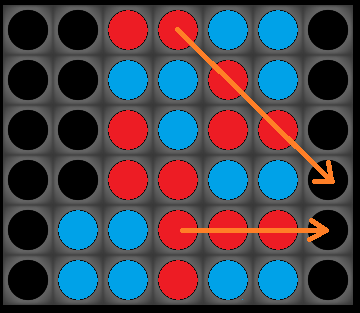
\includegraphics[width=0.4\textwidth]{tablero2turnosfuturo.png}
                \end{center}
                
                En esta situación, la victoria está asegurada para el jugador rojo, y es posible asegurar que ningún jugador implementado, sin importar su optimización, será capaz de anticipar esto. Este tipo de situación inspira quizás replantear si los parámetros que se decidió utilizar son realmente lo suficientemente buenos. Pero en general, también se puede argumentar que es una situación difícil dado que las heurísticas tiene que respetar una cota de complejidad por requerimiento del Trabajo.
                
                \item \textbf{Sobre la optimización de parámetros}: Cuando se generaron los parámetros en primera instancia, estos fueron diseñados dando una prioridad alta al bloqueo de casillas donde el rival tenga un ($C-2$) construido. La razón de darle prioridad a esta situación radica en lo que se llamará \textit{"muerte anticipada"}. Considerar el siguiente ejemplo, en el que el jugador azul realiza su jugada en la columna 5:
                
                \begin{center}
                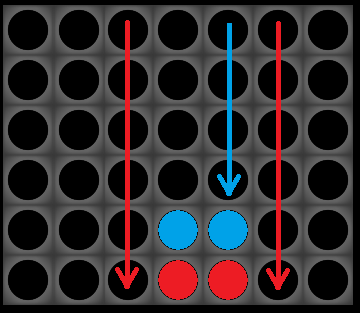
\includegraphics[width=0.4\textwidth]{muerteHorizontal.png}
                \end{center}
                
                En dicha situación, si el azul llega a realizar esa jugada directa, en realidad el jugador rojo puede ganar, debido a que construirá un 3 en línea en el cual trivialmente hay 2 soluciones para ganar.
                
                Si miramos el jugador con la estrategia golosa predeterminada (archivo \texttt{goloso.cpp}), esta situación la defiende; sin embargo, al considerar el jugador optimizado con algoritmo genético, éste convergió a una configuración de parámetros en la cual bloquear un $C-2$ no tiene alta prioridad, resultando en que puede surgir este tipo de escenario donde es derrotado. Este podría ser un motivo factible por el cual este jugador obtuvo resultados ligeramente peores frente al jugador aleatorio en el Experimento 1 (en comparación al jugador Goloso).
                
                Para intentar solventar esto, podríá ser de utilidad reevaluar la función de \textit{fitness}; una buena idea sería armar jugadores triviales que siempre jueguen en este escenario, para que inmediatamente los jugadores que se estén optimizando se vean forzados a jugarlo bien, (o bien  tener un puntaje de \textit{fitness} pésimo, y ser consecuentemente descartados). Sin embargo, el alcance del Trabajo llegó hasta aquí, ya que aún queda más experimentación, y las posteriores conclusiones.
                
    \end{itemize}
    
    
    \subsection{Experimento 3: Evolución del \textit{fitness} en el algoritmo genético}
    
    Para este tercer experimento, se centrará la atención en el jugador cuyos parámetros son optimizados usando el algoritmo genético explicado en la sección 4. de este informe. Como ya se mencionó, la idea en la que se basa un algoritmo genético es en mejorar iterativamente una población inicial de individuos, a partir de evaluar su aptitud (\textit{fitness}), y realizar cruzas y mutaciones genéticas. Por lo tanto, resulta razonable afirmar que los valores de \textit{fitness} de los individuos (es decir, los valores de los parámetros) sufrirán una evolución con el paso de las generaciones.
    
    Esto último da lugar a un experimento, cuyo objetivo es observar de qué manera cambia el \textit{fitness} de los individuos a medida que pasa el tiempo, y transcurren más generaciones. Para eso, se consideró un jugador optimizado con algoritmo genético, con las mismas características usadas en ocasiones anteriores (usando la función de \textit{fitness} \textbf{Puntaje}, la operación de \textit{crossover} \textbf{Moneda}, el mutador \textbf{Normal} y el método de selección \textbf{Mejores}). Luego, en base a una población inicial, se ejecutó el algoritmo durante 100 generaciones, y se calculó el \textit{fitness} promedio de los individuos de cada generación.
    
    Dicho proceso dio lugar a resultados que fueron plasmados en el siguiente gráfico:
    
    \begin{center}
    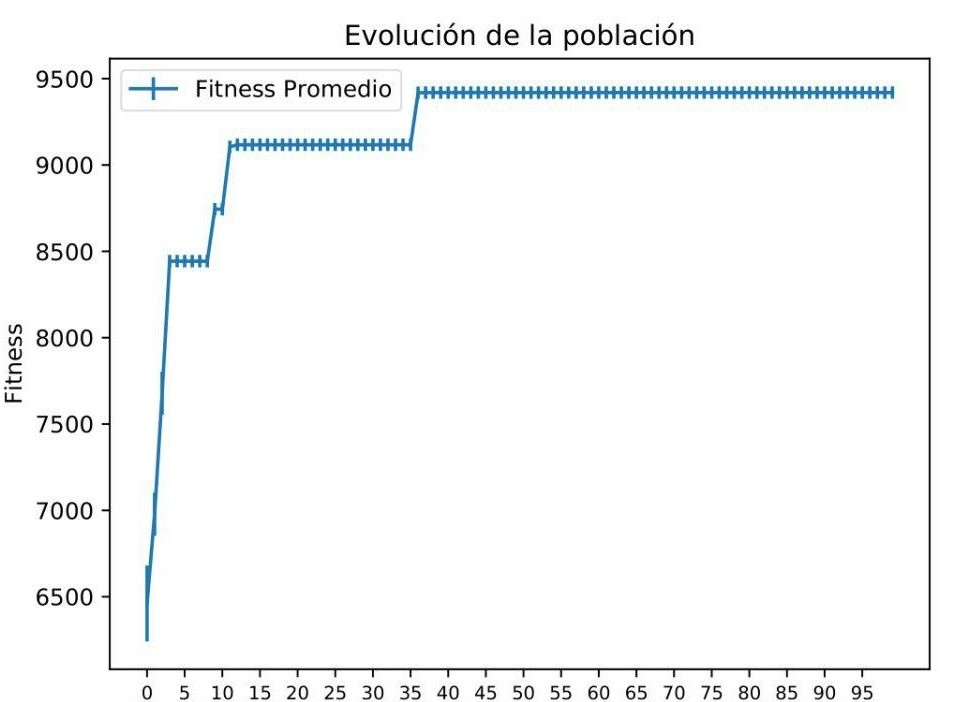
\includegraphics[width=0.7\textwidth]{Evolucion_Genetico.jpg}
    \end{center}
    
    En el eje $x$, se pueden ver las generaciones transcurridas; y en el eje $y$, los valores de \textit{fitness}. La gráfica azul corresponde al \textit{fitness} promedio en cada población, calculada mediante el método \textbf{Puntaje}. \\[3pt]
    
    \underline{Análisis de los resultados:} 
    Es posible ver como durante las primeras 10 o 15 generaciones, el \textit{fitness} crece a un ritmo muy acelerado. Esto tiene sentido, pues teniendo en cuenta que los parámetros iniciales fueron generados aleatoriamente, es razonable que durante las primeras iteraciones del algoritmo haya mucho margen para mejorar los valores asignados. Luego, hay una clara meseta hasta aproximadamente la generación número 35, en la que el algoritmo no pudo encontrar formas de mejorar los genes de los individuos.
    Sin embargo, se da un repentino crecimiento (quizá debido a una mutación que supuso que la población no se estancase en un máximo local), que deriva en una nueva meseta más larga, que se mantiene durante todas las generaciones subsiguientes que fueron observadas.
    Es posible que luego de más generaciones el \textit{fitness} volviese a mejorar, sobre todo teniendo en cuenta que las secciones constantes del gráfico van haciéndose cada vez más largas; pero por cuestiones de tiempo, pareció razonable ejecutar el algoritmo por 100 iteraciones.
    En conclusión, la idea intuitiva de que el \textit{fitness} promedio de los individuos debería aumentar a lo largo del tiempo fue confirmada por el experimento, mostrando que el funcionamiento del algoritmo genético es, tal vez no óptimo, pero sí acertado.




\newpage

%----------------------------------------------------------------------------------------------------------


\section{Conclusiones y trabajo futuro}

Durante el desarrollo de este trabajo práctico, se consiguió realizar un acercamiento a técnicas heurísticas y metaheurísticas, para optimizar la elección de los valores asignados a los parámetros, en el contexto de la resolución de un juego de mesa clásico, utilizando una computadora. De todo esto, se pueden formular ciertas afirmaciones, comentarios y pensamientos finales, a los que se arribó luego de implementar los algoritmos, y \textit{mover} los parámetros analizando las consecuencias.

Por ejemplo, es claro, después de analizar el desempeño de los jugadores implementados, que es de gran relevancia pensar detenidamente tanto qué parámetros se consideran, como el valor que se les va a asignar, aplicando lógica y el \textit{sentido común} que se tiene por conocer como funciona el \textit{4 en línea}. El peso elegido para los parámetros es especialmente importante para obtener buenos resultados con un jugador goloso, pues la calidad de sus jugadas va a depender fuertemente de eso.

Respecto a los parámetros elegidos en este Trabajo, es importante observar que se trató de igual manera las líneas horizontales, verticales y diagonales. Es decir, para el jugador es igual puntuar un cierto valor en línea horizontal, que uno en vertical; lo cual no necesariamente se corresponde con un escenario real, pues por ejemplo, en un \textit{4 en línea}, tres fichas alineadas verticalmente siempre pueden ser neutralizadas por el oponente. En cambio, si hay tres alineadas de manera horizontal, puede ocurrir que no sea posible bloquear todas las maneras de obtener cuatro fichas alineadas. La decisión de tratar a todas estas alternativas por igual fue tomada únicamente en pos de mayor simpleza en la implementación; sin embargo, sería interesante \textit{jugar} con los valores de los parámetros para plasmar efectivamente las diferencias que se mencionarion, e intentar observar si un jugador obtiene mejores resultados de esta manera.

En cuanto al \textit{grid-search}, queda como trabajo pendiente a futuro realizar una búsqueda local como las que se estudió en clase, para poder explorar muchos más valores para los diferentes parámetros, cosa que, por cuestiones de tiempo, no fue posible lograr.

Este Trabajo también sirvió como punto de contacto con los algoritmos genéticos, hoy muy célebres debido al auge del \textit{machine learning}. En cuanto al algoritmo genético desarrollado, resulta de vital importancia dar con una buena función de \textit{fitness}, ya que es la que definirá, en mayor medida, el funcionamiento de la metaheurística; esto es así, pues, por ejemplo, puede darse la situación de haber elegido parámetros que representen bien la información que debe tener el algoritmo para ser exitoso, y aún así, si la función de \textit{fitness} definida no fue lo suficientemente \textit{buena}, puede terminar convergiendo a valores que no obtengan buenos resultados en la práctica. Asimismo, una mala elección de los parámetros incrementa la dificultad a la hora de evaluar la aptitud de los individuos.

Siguiendo con el algoritmo genético, a la hora de definir \textit{crossovers} y \textit{mutaciones}, varias veces se ha dado la situación en que las generaciones de individuos venideras no son lo suficientemente \textit{inteligentes}, a pesar de haber seleccionado a los $k$ mejores ejemplares de la población para que se reproduzcan. Esto es, más allá de que los $k$ mejores sean incluidos en la siguiente generación, ocurrió a menudo que se generaron crías y mutaciones a partir de ellas, las cuales luego comenzaron a perder los enfrentamientos frecuentemente. La conclusión que se puede obtener de este escenario es que los valores de los parámetros convergieron demasiado rápido, lo que puede significar que las generaciones subsiguientes no sean muy \textit{buenas}.

Por último, otro aspecto que influye considerablemente sobre la calidad de los resultados del algoritmo genético son las características de la población inicial. En el caso del algoritmo implementado, esta fue generada de una sola manera: aleatoriamente. Por esto, seguramente habría enriquecido la experimentación (y quizás también mejorado los resultados) el probar con otras formas de generar esta población inicial. Todas estas cuestiones mencionadas quedan pendientes como trabajo a ser realizado en un futuro.

En resumen, y para concluir, este Trabajo fue útil en el sentido de que se exploraron maneras de resolver un problema que no son exactas, como sí lo eran las que se habían estado estudiando y utilizando hasta el momento. Por lo tanto, se podría afirmar que resultó exitoso en abrir las puertas a otras formas de implementar algoritmos, que además, tienen diversos usos en diferentes campos de esta disciplina.







%----------------------------------------------------------------------------------------------------------

\end{document}
